\section{Endliche Körper}
%
%
%
\subsection{Satz:}
Zu jedem endlichen Körper $L$ existiert eine Primzahl $p$ so dass gilt:
\begin{enumerate}[label={(\alph*)}]
	\item $K = \mathop{\underbrace{\{1+1+ \dotsc +1\}}}\limits{k\text{-mal}}|k \in \mathbb{N}$ ist ein Teilkörper von $L$ 
		isomorph zu $\mathbb{Z}/p\mathbb{Z}$.
	\item $L$ ist ein $K$-Vektorraum. Insbesondere gilt $|L| = p^{n}$ für $n = dim_{k}L$
	\item $\mathop{\underbrace{a+ \dotsc +a}}\limits_{p\text{ mal für jedes } a \in L} = 0$
\end{enumerate}
Beweis:
\begin{enumerate}[label={(\alph*)}]
	\item Betrachte: $\varphi :\mathbb{Z} \rightarrow L$\\
				.\qquad \quad \qquad $z \rightarrow \mathop{\underbrace{1+ \dotsc + 1}}\limits_{z\text{ mal}}$\\
				$\varphi$ ist ein Ringhomomorphismus. Sei Kern $\varphi = n \mathbb{Z}$ (mit $n\in\mathbb{N}$)\\
				$\varphi^{-1}$: Bild $\varphi \rightarrow \mathbb{Z}/n\mathbb{Z}$\\
				.\qquad \qquad $a \rightarrow \varphi^{-1}(a)=k+m\mathbb{Z}$ wo $\varphi(k)=a$.
				$\varphi^{-1}$ ist ein bijektiver Ringhomomorphismus. \\
				$\Rightarrow K =$ Bild $\varphi$ ist ein Teilring von $L$ und $K$ und isomorph zu 
				$\mathbb{Z}/n\mathbb{Z}$.\\
				Mit $L$ ist auch $K$ nullteilerfrei $\Rightarrow \mathop{m}\limits_{\mathop{p}\limits^{\Downarrow}}$ 
				ist eine Primzahl.
	\item $L$ ist $k$-Vektorraum, wenn man als Skalarmultiplikation die Multiplikation in $L$ verwendet. \\
		$L \cong K^{n}$ für $n=dim_{K} \ L\Rightarrow |L|=p^{n}$
	\item $\mathop{\underbrace{a+\dotsc + a}}\limits_{p\text{ - mal}}= a \cdot \mathop{\underbrace{(1+ \dotsc 
		+1)}}\limits_{p\text{ - mal}} = a \cdot 0 = 0$
\end{enumerate}
%
%
%
\subsection{Definition:}
Das $p$ in III.5.1 nennen wir die Charakteristik des Körpers $L$. Das $K$ in III.5.1 nennen wir den Primkörper von $L$.
%
%
%
\subsection{Satz:}
Zu jeder Primzahlpotenz $p^{n}$existiert ein endlicher Körper $GF(p^{n})$ mit $p^{n}$ Elementen. $GF(p^{n})$ ist Menge aller Nullstelle des Polynoms.
\begin{equation*}
x^{p^{n}} -x \in (\mathbb{Z}/p\mathbb{Z})[x]
\end{equation*}
\textbf{Beweis:}\\
Wir wenden die Konstruktion III.4.8 so lange auf irreduzible Faktoren von $x^{p^{n}} -x$ an, bis wir einen endlichen Körper $M \supseteq \mathbb{Z}/p\mathbb{Z}$ gefunden haben, so dass $x^{p^{n}} -x$ in $M[x]$ in Linearfaktoren zerfällt. Setze $L=\{a\in M|a^{p^{n}}=a\}$
\begin{description}
	\item[Zeige:] $L$ ist ein Teilkörper von $M$. Betrachte dazu $a,b \in L$
	\item[-] $(a \cdot b)^{p^{n}} = a^{p^{n}} \cdot b^{p^{n}} = a \cdot b \Rightarrow a \cdot b \in L$
	\item[-] $(a+b)^{p^{n}} =^{\text{**}} a^{p^{n}}+b^{p^{n}}=a+b \Rightarrow a+b \in L$
\end{description}
**\textbf{Behauptung:} $(x+y)^{p} = x^{p}+y^{p}$ für alle $x,y \in M$. $\mathop{\underbrace{(x+y)\cdot \dotsc \cdot (x+y)}}\limits_{p\text{ - mal}}$ ist die Summe von Termen der Form $x^{k}\cdot y^{p-k}$. Dabei tritt $x^{k}\cdot y^{p-k}$ sof oft auf, wie ich aus den $p$ Klammern $k$ Klammern wählen kann, um von dort das $x$ zu rekrutieren. Also genau:\\
$\frac{p\cdot(p-1)\cdot(p-2)\cdot \dotsc \cdot(p-k+1)}{k!}$ Möglichkeiten. Ist $1\leq k \leq p-1$, so bleibt die Primzahl $p$ beim kürzen stehen.\\
 III.5.1 (c) $\Rightarrow$ Es überleben nur dei Terme $x^{p}\cdot y^{0}$ und $x^{0} \cdot y^{p}$ in der Summe.\\
Zeige: $|L,| = p^{n}$ Dazu: die Linearfunktionen $x-a (a \in L)$ von $x^{p^{n}}-x$ in $M[x]$ treten mit Vielfachheit 1 auf. \\
Formale Ableitung: $\mathop{p^{n} \cdot x^{p^{n}-1}}\limits_{\mathop{p^{n}\text{ - fache der Summe der }1\text{ in }M}\limits^{\uparrow}} = 0 \cdot x^{p^{n}} -1 =\mathop{-1}\limits_{\mathop{\text{kein Platz für Linearfaktor }x-a}\limits^{\uparrow}}$\\
\qquad\\
Wende nun Blatt 8 an. /* Aufgabe formale Ableitung */ $\square$
%
%
%
\subsection{Bewertung:} 
Man kann zeigen:
\begin{enumerate}[label={(\alph*)}]
	\item Es gibt genau einen Kröper mit $p^{n}$ Elementen (bis auf Isomorphie)
	\item In $GF(p^{n})$ existiert ein $a \neq 0$ mit $GF(p^{n})=\{a,a^{2},\dotsc, 
			a^{p^{n}-2}\}$ (d.h. $GF(p^{n})^{\times}$ \\
			$\mathop{\cong}\limits_{\text{als Gruppe}}
			(\mathbb{Z}/(p^{n}-1)\mathbb{Z})^{+}$)
\end{enumerate}
%
%
%
\subsection{Beispiel:}
$GF(9) = K[x]/fK[x]$ wo $K = K/3\mathbb{Z}$ und $f=x^{2}+2x+2$\\
$G \neq (9)^{\times} \cong ( \mathbb{Z}/8\mathbb{Z})^{+} \leftarrow$ erzeugt von den invertierbaren Elementen teilfremd zu 8 $\rightarrow$ 4. Stück\\
\begin{equation*}
x \neq 1, x^{2}=x+1 \neq 1, x^{4} = (x+1)^{2}=2 \neq 1 \Rightarrow GF(9)
\end{equation*}
erzeugt von:
\begin{equation*}
x, x+2, 2x, 2x+1
\end{equation*}
(sogenannte primitive Elemente)

\begin{figure} [H]
\centering 
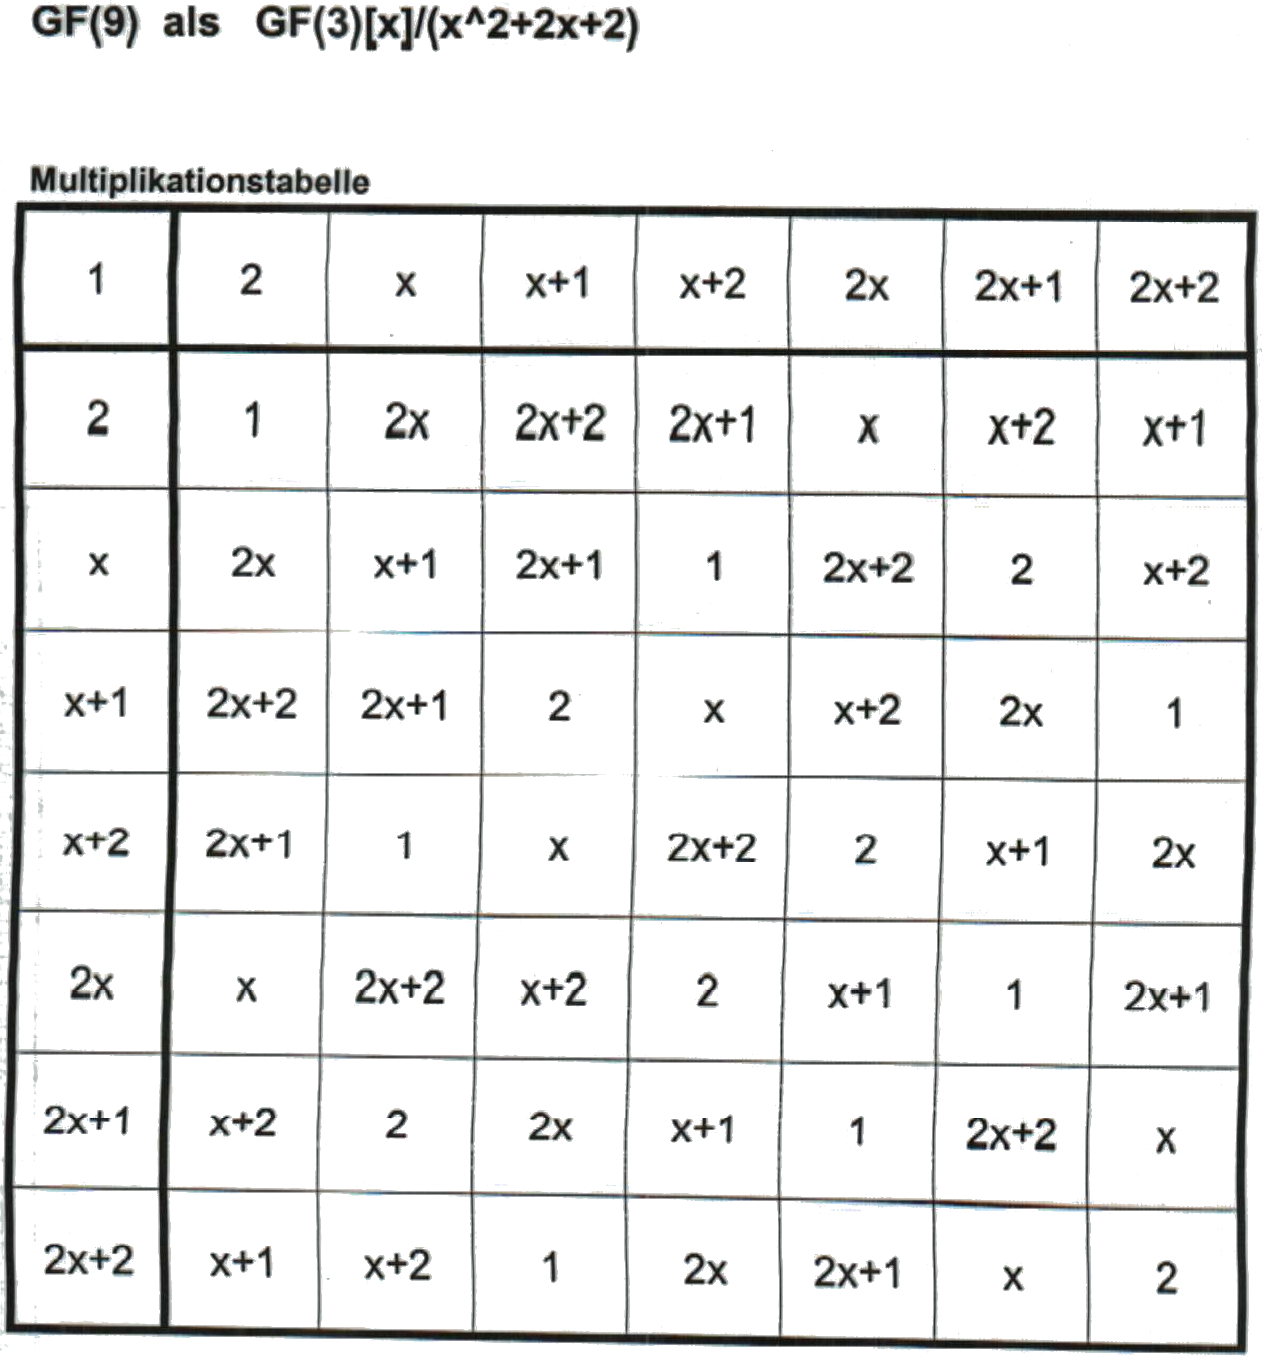
\includegraphics[width=10cm, height=10cm]{mainmatter/chapter3/pics/multitabelle.png}
\caption{Eine Multiplikationstabelle} 
\end{figure}
